\usepackage{amsthm}
\usepackage{booktabs}
\usepackage[T1]{fontenc}
\usepackage[margin=1in]{geometry}
\usepackage{mathtools}
\usepackage{microtype}
\usepackage{minted}
\usepackage{natbib}
\usepackage{newpxmath}
\usepackage{newpxtext}
\usepackage{rgalg}
\usepackage{thmtools}
\usepackage{tikz}
\usepackage{xcolor}

\usepackage{hyperref}

\usepgflibrary{arrows}
\usetikzlibrary{matrix}

\definecolor{darkblue}{rgb}{0,0,0.4}
\definecolor{darkgreen}{rgb}{0,0.4,0}
\hypersetup{colorlinks,linkcolor=darkblue,citecolor=darkblue,urlcolor=darkblue}

\usemintedstyle{tango}
\newminted{c}{linenos}
\newminted{java}{linenos}

\renewcommand*\.[1]{{\sf#1}}

\newcommand*\lecture[1]{
  \centerline{
  \framebox[1.05\textwidth]{\vbox{
    \hbox to\textwidth{{\bf CO527: Operating Systems}\hfil Spring 2017}
    \vspace{3ex}
    \hbox to\textwidth{\hfil\Large\bf#1\hfil}
    \vspace{3ex}
    \hbox to\textwidth{\it Radu Grigore\hfil}
  }}}
  \vspace{5ex}\par
}

\newcommand*\asgn\coloneqq
\newcommand*\df\emph
\newcommand*\todo[1]{\marginpar{\raggedright\tiny\color{darkgreen}TODO: #1\par}}
\newcommand*\defeq\coloneqq

\declaretheorem{theorem}
\declaretheorem[sibling=theorem]{lemma}

\title{Operating Systems Concepts}
\author{Radu Grigore}

\begin{document}
\lecture{Virtual Memory}

% must cover:
% - page-to-frame mapping is n-to-1

\section*{Process Address Space}

% plan: sparse, mmap, vmareas, typical structure, shared parts

A process is what we colloquially call a program, roughly.
But, there are subtle nuances.
As users, we tend to define a program by what it does for us.
For the operating system,
  what matters about a process is what resources it gets.
There are two main resources: processor time, and memory space.
We will talk about processor time later.
Now we talk about the memory space available to a process.

Each process gets its own memory.
This memory is sometimes called \df{virtual memory},
  when we want to emphasize that it is not a physical entity;
other times it is called a \df{process address space},
  when we want to emphasize that it is associated to one process.
Since distinct processes have isolated, distinct address spaces,
  a crash of one process will not bring down other processes.
This isolation is partly implemented in the operating system,
  and partly implemented in the processor.

Now let us focus on the address space of one process.
On my computer,
  the size of the virtual memory (of each process) is $2^{48}$~bytes,
  and the size of the physical memory (of the computer) is $2^{34}$~bytes:
\begin{verbatim}
  rg@rg-2016:notes$ cat /proc/cpuinfo | grep address | head -1
  address sizes	: 39 bits physical, 48 bits virtual
  rg@rg-2016:notes$ cat /proc/meminfo | head -1
  MemTotal:       16321420 kB
\end{verbatim}
The special files \.{/proc/cpuinfo} and \.{/proc/meminfo}
  contain information about the processor and about the memory, respectively.
From \.{cpuinfo},
  we see that the processor \emph{can} handle physical memory
    of up to $2^{39}$~bytes (512~GiB),
  and offers a virtual memory of size $2^{48}$~bytes (256~TiB).
From \.{meminfo},
  we see that the physical memory is only $2^{34}$~bytes (16~GiB).

If a process thinks that 256~TiB are available,
  it might try to use more than 16~GiB\null.
In that case, the operating system will try to use the hard disk.
If the process does not access too often the data that the operating system
  happens to move to the hard disk,
  then all is OK\null.
But, it is also possible that the process will try to actively use
  more than 16~GiB,
  which will force the operating system to keep moving information
    between the physical memory (RAM) and the hard disk.
In that case the user sees that the hard disk is used continuously,
  and all the programs on the system seem to grind to a halt.
We call this \df{thrashing}.

In summary,
  if a process tries to use more than the available physical memory,
  the system will become unusable.
Conversely,
  on a usable system,
  each process uses less memory than it is available physically.
(These are not hard rules,
  because much depends on the pattern of memory accesses.
For example,
  if a process writes a byte at some virtual address
  but then never touches it again,
  then that byte will likely move to the hard disk and stay there.
So, from the point of view of our discussion,
  it should not really count as being used;
  but, technically, it is used.)
The bottom line is this:
  We should expect the process address space to be sparse.
On my computer,
  even if a process address space is 256~TiB in size,
  I expect that less than 16~GiB of those are used.
That is, less than $0.0062\%$.

\begin{figure}
\begin{center}
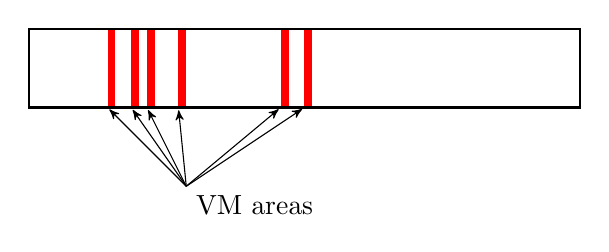
\begin{tikzpicture}
  \foreach \x in {1,1.3,1.5,1.9,3.2,3.5} {
    \fill[red] (\x,0) rectangle (\x+0.1,1);
    \draw[->,>=stealth',shorten >=1pt] (2,-1) -- (\x,0);
  }
  \node[below right] at (2,-1) {VM areas};
  \draw[thick] (0,0) rectangle (7,1);
%  \node[above right] at (0,1) {virtual process address space};
\end{tikzpicture}
\end{center}
\caption{Virtual Process Address Space}
\label{fig:vm}
\end{figure}

\autoref{fig:vm} illustrates that the process address space is sparse.
The used parts --- the thin red lines --- are called \df{VM areas}.
Before using a part of its address space,
  a process must announce the operating system by calling function \.{mmap};
for example,
\begin{ccode}
  mmap(0, length, prot, flags, -1, 0);
\end{ccode}
We say that that a VM area was \df{mapped}.
The process may also inform the operating system that it intends
  to not use a certain portion of the address space,
  by calling \.{munmap}.
When a process is created,
  certain areas are mapped automatically:
  an area for the call stack,
  an area for libraries such as the C standard library,
  an area for the heap,
  a couple of areas for global variables (initialised or not),
  an area for the code of the process being executed.
\todo{Add a picture with the standard areas.}
Moreover, some of these areas can grow or shrink.
For example,
  the system call \.{brk} can be used to grow or shrink the heap.
A call to \.{malloc} will typically try to use the heap area,
  and may result in a call to \.{brk} behind the scenes.
What \.{brk} does is similar to \.{mmap} and \.{munmap}.
We have so many types of areas,
  and different ways to map and unmap them,
  that this becomes quickly overwhelming to remember.
The main point is that the operating system has a data structure
  that keeps track of which virtual memory areas are in use.
This data structure is essentially a list of intervals:
\[
  [a_1,b_1),\; [a_2,b_2),\;\ldots,\;[a_n,b_n)
\]
An address is in use if it is inside one of these intervals/areas.

\smallskip

Different areas have different properties.
For example, areas that contain code are generally marked as \emph{read-only}.
Areas that correspond to library code,
  such as the standard C library,
  are \emph{shared} among many process address spaces,
    meaning that they are not copied multiple times in the physical memory.
Properties such as read-only and shared are specified
  in the \.{prot} and \.{flags} arguments of \.{mmap}.
\todo{Explain how some areas are backed by files.}
To understand what some of these properties do,
  we need to look in some detail at how virtual addresses
  are translated into physical addresses.

\section*{Translating Addresses}

% why pages, page tables

Each memory access performed by a process in user space uses virtual addresses;
  that is, the process only knows about its address space.
However, that memory access must go to some address in the physical memory.
How do we track the correspondence between virtual and physical addresses?
A simple option would be to keep a list of pairs
\[
  (x_1,y_1),\; (x_2,y_2),\; (x_3,y_3), \ldots
\]
meaning that virtual address $x_i$ maps to physical address $y_i$ for all~$i$.
What's wrong with this?
One issue is that we'd need a lot of space to keep this list.
This is not a `let us not waste memory' issue:
  this is a `there is no way we have that much memory issue'.
The standard solution to this problem
  is to slice the memory into slices of equal sizes.
We call slices in the virtual memory \df{pages},
  and we call slices in the physical memory \df{frames}.
(The terminology is not completely standard.
  For example, one may also say `virtual page' instead of `page',
    and `physical page' instead of `frame'.)
Pages and frames have the same size: one page exactly fits in one frame.
This size is usually 4~KiB or 8~KiB\null.
Now we can keep a list of pairs, exactly as before,
  but now we only list virtual addresses that point at the beginning of pages,
  and they'll be paired with physical addresses that point at the beginning of frames.
The resulting data structure, which maps pages to frames,
  is called \df{page table}.
This data structure is used by the processor while running in user mode.
So, we should expect the operating system to need some architecture dependent
  code to access the page table.

\smallskip

For and example,
  consider a computer with $48$~bit virtual addresses and $4$~KiB page size.
Suppose the virtual address is ${\tt ba9876543210}_{16}$.
The position within the page is given by the last $12$~bits:
  ${\tt210}_{16}$.
The page number is given by the other $36$~bits:
  ${\tt ba9876543}_{16}$.
Suppose now that there are $4$~GiB of physical RAM,
  and the page table contains the mapping
  ${\tt ba9876543}_{16} \mapsto {\tt edcba}_{16}$.
Then the corresponding physical address is
  ${\tt edcba210}$.
In general,
\begin{align}
p &= {\it page\_table}\biggl(\biggl\lfloor\frac{v}{s}\biggr\rfloor\biggr) \cdot s
  + v \bmod s
  \label{eq:translation}
\end{align}
where $p$~is the physical address,
  $v$~is the virtual address,
  and $s$~is the (fixed) page size.
Often, $s=2^k$ for some~$k$, which means one can use this C (and Java) code:
\begin{ccode}
  p = (page_table[v >> k] << k) + (v & ((1 << k) - 1));
\end{ccode}
This translation, from a virtual address into a physical address,
  needs to be done every time a process accesses memory.
\todo{say what needs to hold for the shifts to do the same in C/Java}
This translation is therefore performance critical,
  which is why most systems have hardware support for it:
  MMU ({\bf m}emory {\bf m}anagement {\bf u}nit).

Conceptually,
  the page table is a function from page numbers to frame numbers.
A simple representation for such a function is a set of mappings; for example,
\begin{align*}
  \{
  {\tt ba9876543}_{16} \mapsto {\tt edcba}_{16},\;
  {\tt ba789abcd}_{16} \mapsto {\tt 12345}_{16},\;
  {\tt 111111111}_{16} \mapsto {\tt 22222}_{16},\;
  \dots
  \}
\end{align*}
Given the left-hand side of a mapping, one wants to quickly find the right-hand side.
Even with hardware support, this operation is expensive.
Note that one cannot simply have an array indexed by the page number:
  that would be too big.
%In the example above, we'd need an array of size~$2^{36}$.
Instead, one uses a multi-level page-table:
\begin{align*}
  \Bigl\{
    {\tt ba9}_{16} \mapsto
      \bigl\{
        {\tt 876}_{16} \mapsto \{ {\tt 543}_{16} \mapsto {\tt edcba}_{16}\},\;
        {\tt 89a}_{16} \mapsto \{ {\tt bcd}_{16} \mapsto {\tt 12345}_{16}\}
      \bigr\},\;
    {\tt 111}_{16} \mapsto
      \bigl\{
        {\tt 111}_{16} \mapsto \{ {\tt 111}_{16} \mapsto {\tt 222}_{16} \}
      \bigr\},\;
    \dots
  \Bigr\}
\end{align*}
In this example, we first lookup the most significant $12$~bits of the page number,
  and the result is a nested page table;
  in the nested page table we lookup the next $12$~bits of the page number,
  and the result is again a nested page table;
  finally, in the doubly-nested page table we lookup the last $12$~bits of the page number,
  and the result is the frame number.
Thus,
  we can implement the top-most level of the page table as an array of size~$2^{12}$.
The drawback is that we need several lookups in such arrays: three.

To speed up the address translation even more,
  the hardware takes advantage of locality of reference.
Not only memory accesses exhibit locality of reference,
  but also lookups in the page table.
Here is one way to understand this concept.
Suppose that the (nested) page table contains $N$~mappings.
Suppose that doing $N$~lookups takes $1$~second.
Now we do an experiment:
  we sample at random $1$~second from the operation of the page table.
Because of our assumptions, in this time the MMU did roughly $N$~lookups.
Now we look at how many \emph{distinct} mappings where looked up.
Let's say the number is~$M$.
Locality of reference means that often it is the case
  that $M$ is \emph{much} smaller than~$N$.
Clearly, it's worth caching the page table!

Indeed, the MMU usually contains a piece of hardware that caches page table entries
  and is called TLB ({\bf t}ranslation {\bf l}ookaside {\bf b}uffer).
The TLB is implemented as a content addressable memory.
This means that the TLB tracks a set of mappings,
  can do fast (constant time) lookups,
  and yet it does not use an array.
Instead, the hardware is designed in a completely different way.
Wait a minute --- you might say ---
  if such a thing is possible to implement in hardware,
  why don't we use it to store the whole set of mappings?
The answer is that content addressable memories are expensive.
Simply put, we know how to implement TLBs,
  but their size is limited by what we can achieve in hardware.

\smallskip

Note that each process has it own address space and therefore its own page table.
The page table is set up by software:
  it is the operating system that decides its content.
The page table is used by hardware:
  the processor regularly performs address translations while running in user mode.
If the straightforward translation fails,
  for example because a page was accessed but it has no frame,
  then the processor passes control to a \df{page fault handler},
    which is a part of the operating system that should fix the problem.
The basic mechanism from~\eqref{eq:translation}
  can easily be suplemented with other functionality.
The page table entry for one page can contain more than just the frame number.
It can contain whether that page should or should not be writable;
  it can contain whether that page is dirty
    (that is, whether it has an identical copy on the hard disk);
  it can contain whether that page contains code.




\todo{Add a section about page allocation.}
%\section*{Page Allocation}

\section*{Exercises}

\begin{enumerate}
\item
  Skim through `\.{man 2 mmap}'.
\item
  $\blacktriangleright$
  The text says that keeping a list of (virtual address, physical address) pairs
    would require way too much memory.
  How much, exactly?
\item
  $\blacktriangleright$
  The mapping virtual--physical address is
    (a)~one-to-one,
    (b)~one-to-many,
    (c)~many-to-one, or
    (d)~many-to-many?
\item
  What is the page size on your computer?
  [Hint: See `\.{man 2 getpagesize}'.]
\item
  $\blacktriangleright$
  The virtual memory subsystem of the operating system
    implements a mechanism called COW: copy-on-write.
  Can you guess from the name what it does?
  If not, can you google it?
\item
  The Linux kernel has a \.{vm\_area\_struct}
    for each mapped area within a virtual address space.
  If \.{mmap} is asked to map a new area,
    and no hint is given as to where the new area should be placed,
    then how does Linux chose the location?
  [Hint: See the function \.{unmapped\_area} in the file \.{mm/mmap.c}.]
\item
  A VM area is represented in the kernel by \.{vm\_area\_struct},
    which is defined in \.{include/linux/mm\_types.h}.
  Take a look at that code.
  Notice that an interval tree is mentioned.
  Further relevant code is in \.{mm/interval\_tree.c}.
  The \href{https://en.wikipedia.org/wiki/Interval_tree}{Interval tree}
    article on Wikipedia may be useful.
  What is the \.{anon\_vma} list?
  What is the \.{i\_mmap} tree?
\item
  Each VM area has a custom set of operations;
    see \.{vm\_operations\_struct} in \.{include/linux/mm.h}.
  One of these operations is the page fault handler.
  Why might we want different VM areas to have different fault handlers?
\item
  In the Linux kernel, page allocation is done using the buddy system.
  Look at the implementation in \.{mm/page\_alloc.c}.
  An older version of the implementation is described
    \href%
      {https://www.kernel.org/doc/gorman/html/understand/understand009.html}%
      {here}.
\item
  Take a look at the (architecture dependent) code for handling page tables.
  For example, see \.{arch/x86/mm/pgtable.c}.
\item
  Look at [4] to see how content-addressable memory is implemented.
\end{enumerate}

\section*{References}

\begin{itemize}
\item[{[1]}]
  Duarte,
  \href%
    {http://duartes.org/gustavo/blog/post/how-the-kernel-manages-your-memory/}%
    {How the Kernel Manages Your Memory}.
\item[{[2]}]
  Vavrusa,
  \href{http://marek.vavrusa.com/c/memory/2015/02/20/memory/}%
    {What a C programmer should know about memory}.
\item[{[3]}]
  The \.{mm/} directory of the Linux kernel version~4.2.0.
\item[{[4]}]
  Pagiamtzis and Sheikholeslami,
  \emph{Content-Addressable Memory (CAM) Circuits and Architectures:
    A Tutorial and Survey},
  2005.
\end{itemize}


\end{document}

% vim:spell:spelllang=en_gb:
